\chapter{Opis projektnog zadatka}
		

		Ideja našeg projekta je ostvariti aplikaciju koja će omogućiti korisniku da pregledava, rezervira i naplaćuje parkirna mjesta za automobile i bicikle.
		Aplikacija to ostvaruje na način da prilikom njezinog otvaranja prikazuje korisniku kartu nad kojom korisnik može birati željeno odredište, tip vozila koje koristi te trajanje parkiranja. Nakon svih odabira, na karti mu se iscrtava najbrža ruta do slobodnog parkirališnog mjesta te ako je mjesto slobodno, ono se rezervira. Parkirališta za bicikle nemaju ucrtana pojedinačna mjesta te se ne rezerviraju ni naplaćuju, već aplikacija jedino prati ukupan broj slobodnih mjesta.
		Za računanje najbližeg dostupnog parkirališnog mjesta aplikacija koristi OSRM, što je kratica za Open Source Routing Machine. Riječ je o modernom C++ algoritmu za usmjeravanje koji se koristi za izračunavanje najkraćeg puta u cestovnom prometu. 
		
	    \noindent Aplikacija koristi API za više funkcija:
		\begin{packed_item}
			\item implementacija novčanika u koji korisnik uplaćuje sredstva
			\item osvježavanje parkirališnog mjesta radi provjere zauzetosti
			\item dohvaćanje početnih informacija o stanju parkirališnih mjesta pri čemu se koristi overpass API
		\end{packed_item}
		 
		Aplikacija se može pokrenuti bez registracije, no za pristup svim alatima aplikacije, potrebna je registracija. Korisnici koji nisu registrirani mogu na karti vidjeti sva dostupna parkirališta i parkirališna mjesta, ali nemaju informacije u njihovom stanju u stvarnom vremenu. Neregistrirani korisnik koji se želi registrirati šalje zahtjev za registraciju pri čemu ima opciju birati između dvije uloge (voditelj parkirališta i klijent). Za registraciju su potrebni:
		\begin{packed_item}
			\item korisničko ime
			\item ime
			\item prezime
			\item slika osobne
			\item IBAN račun
			\item email adresa
		\end{packed_item}
		
		Za registraciju kao klijent dovoljna je samo potvrda preko email adrese. Ako je riječ o voditelju parkirališta tada je potrebna i potvrda administratora.
		
		  \underbar {\textit {Klijent}} otvaranjem aplikacije dobiva pregled nad kartom te odabire lokaciju odredišta, tip vlastitog vozila, i trajanje parkiranja. Klijent može rezervirati parkirališno mjesto na dva načina. Može prvo označiti parkirališna mjesta koja mu odgovaraju te mu tada aplikacija nudi moguće termine u kojima će ta mjesta biti slobodna. Druga opcija je da prvo definira odgovarajući termin nakon čega će mu aplikacija prikazati sva parkirališna mjesta koja su slobodna u tom terminu. Aplikacija razlikuje parkirališna mjesta čije su razine različite te korisnik ima mogućnost odabira. Kada je klijent zadovoljan s parkirališnim mjestom, rezervira mjesto na proizvoljno vrijeme ako je slobodno te pri tome ima opciju da napravi rezervaciju ponavljajućom. Klijent jedino može rezervirati mjesto u budućnosti, odnosno, mjesto ne može biti rezervirano u istom datumu u kojem je korisnik otvorio aplikaciju. Plaćanje parkiranja korisnik obavlja tijekom rezervacije ili po dolasku na parkirališno mjesto. Plaćanje se obavlja preko novčanika koji je implementiran unutar aplikacije u koji korisnik može proizvoljno ubaciti novac. 
		
		 \underbar {\textit {Voditelj parkirališta}} ima veće ovlasti od klijenta. On ima dozvolu unijeti podatke o vlastitom parkiralištu koje uključuju:
		  
		  
		 
		 \begin{packed_item}
		 	\item naziv
		 	\item opis
		 	\item fotografija
		 	\item cjenik i sl.
		 \end{packed_item}
		
		\noindent Voditelj nad svojim parkiralištem može individualno ucrtati svako parkirališno mjesto prema vlastitim željama. Nakon što ucrta mjesta, on odlučuje je li mjesto dostupno za rezervaciju. Dodatno, voditelj postavlja i senzor koji služi za dohvaćanje informacije o zauzetosti mjesta. Za svoje parkiralište voditelj određuje cijenu rezervacije ovisnu o vremenu. Voditelj također ima i pristup statističkim podacima o svom parkiralištu. Moguće je promatrati zauzetost cijelog parkirališta te pojedinačnih parkirališnih mjesta kroz vrijeme uz pomoć grafa.
		
		
		\underbar {\textit {Administrator}} aplikacije ima najveće ovlasti i sposoban je vidjeti popis svih registriranih korisnika i njihovih osobnih podataka te im po potrebi može mijenjati osobne podatke.
		
		Motivacija za razvoj ovog projekta dolazi od mnogih prednosti koje aplikacija za parkiranje može donijeti u odnosu na klasičan način rezerviranja i plaćanja parkiranja. Za početak, korištenjem ove aplikacije korisniku se značajno smanjuje vrijeme potrebno za pronalaženje parkirališnog mjesta. Dodatno, plaćanje parkirališnog mjesta može biti izvor frustracije zbog korištenja kovanica i gomilanja sitniša ili zbog potrebe za vađenjem kartice. Aplikacija za taj problem nudi praktično rješenje implementacijom novčanika što omogućuje korisniku da sva svoja plaćanja obavi unaprijed preko mobilnog telefona. Jednostavnost i elegantnost ove aplikacije pomaže i pri smanjenju stresa kod korisnika. Pitanja poput: "Gdje ćemo parkirati?", "Smijem li ja parkirati na ovom mjestu?" ili "Ima li uopće slobodnih mjesta?" više neće biti razlog za brigu jer aplikacija obavlja sve razmišljanje za vas. Problem traženja parkirališnog mjesta u nepoznatom gradu će se svesti na samo par klikova na aplikaciji te će uštedjeti korisnicima i novac budući da neće gubiti vrijeme vozajući se po gradu, tražeći slobodno mjesto. Konačno, aplikacija pridonosi i okolišu jer manje vremena potrošeno na potražnju mjesta za parkiranje znači manje vremena koje trošimo na sagorijevanje goriva.
		
		Neke od aplikacija koje pružaju slična rješenja su:
		\begin{packed_item}
			\item SpotHero
			\item Best in Parking
			\item ParkWhiz
			\item Parkopedia
			\item Way
		\end{packed_item}
		
		Kako bi bolje ilustrirali prednosti koje naša aplikacija ima u odnosu na neke od postojećih rješenja, uzet ćemo kao primjer \textit {SpotHero}. \textit {SpotHero} korisniku prikazuje dostupna parkirališna mjesta u blizini nakon što korisnik upiše adresu na kojoj se nalazi. Korisnik tada može kartu rezervirati i tada dobiva propusnicu koju skenira na parkirališnom mjestu. \textit {SpotHero} omogućuje korisniku mjesečno parkiranje te parkiranje u zračnoj luci. Bitna razlika između naše aplikacije i \textit {SpotHero} je to da kod korištenja \textit {SpotHero-a} korisnik mora odmah definirati termin i vrijeme parkiranja dok naša aplikacija dozvoljava korisniku da prvo označi parkirališna mjesta, a nakon toga mu se nude dostupni termini. Aplikacije se razlikuju i u tome što \textit {SpotHero} ne daje opciju za bicikle, već samo za osobna vozila. Dodatno, \textit {SpotHero} je jedino dostupan u SAD-u i Kanadi.
		
		 \textit {Parkopedia} je još jedna takva slična aplikacija. \textit {Parkopedia} koristi Google Maps kako bi iscrtala najbližu rutu korisniku. Razlika između našeg projekta i ove aplikacije je što \textit {Parkopedia} zahtijeva da se prvo unese adresa odredišta nakon čega nudi popis dostupnih parkirališta. \textit {Parkopedia} na prikazu karte daje opciju između prikazivanja parkirališnih mjesta na ulici i u garaži. Kao i kod \textit {SpotHero-a}, \textit {Parkopedia} ne nudi opciju za bicikle te pretraga prvo po terminu parkiranja nije moguća.
		
		\begin{figure}[H]
			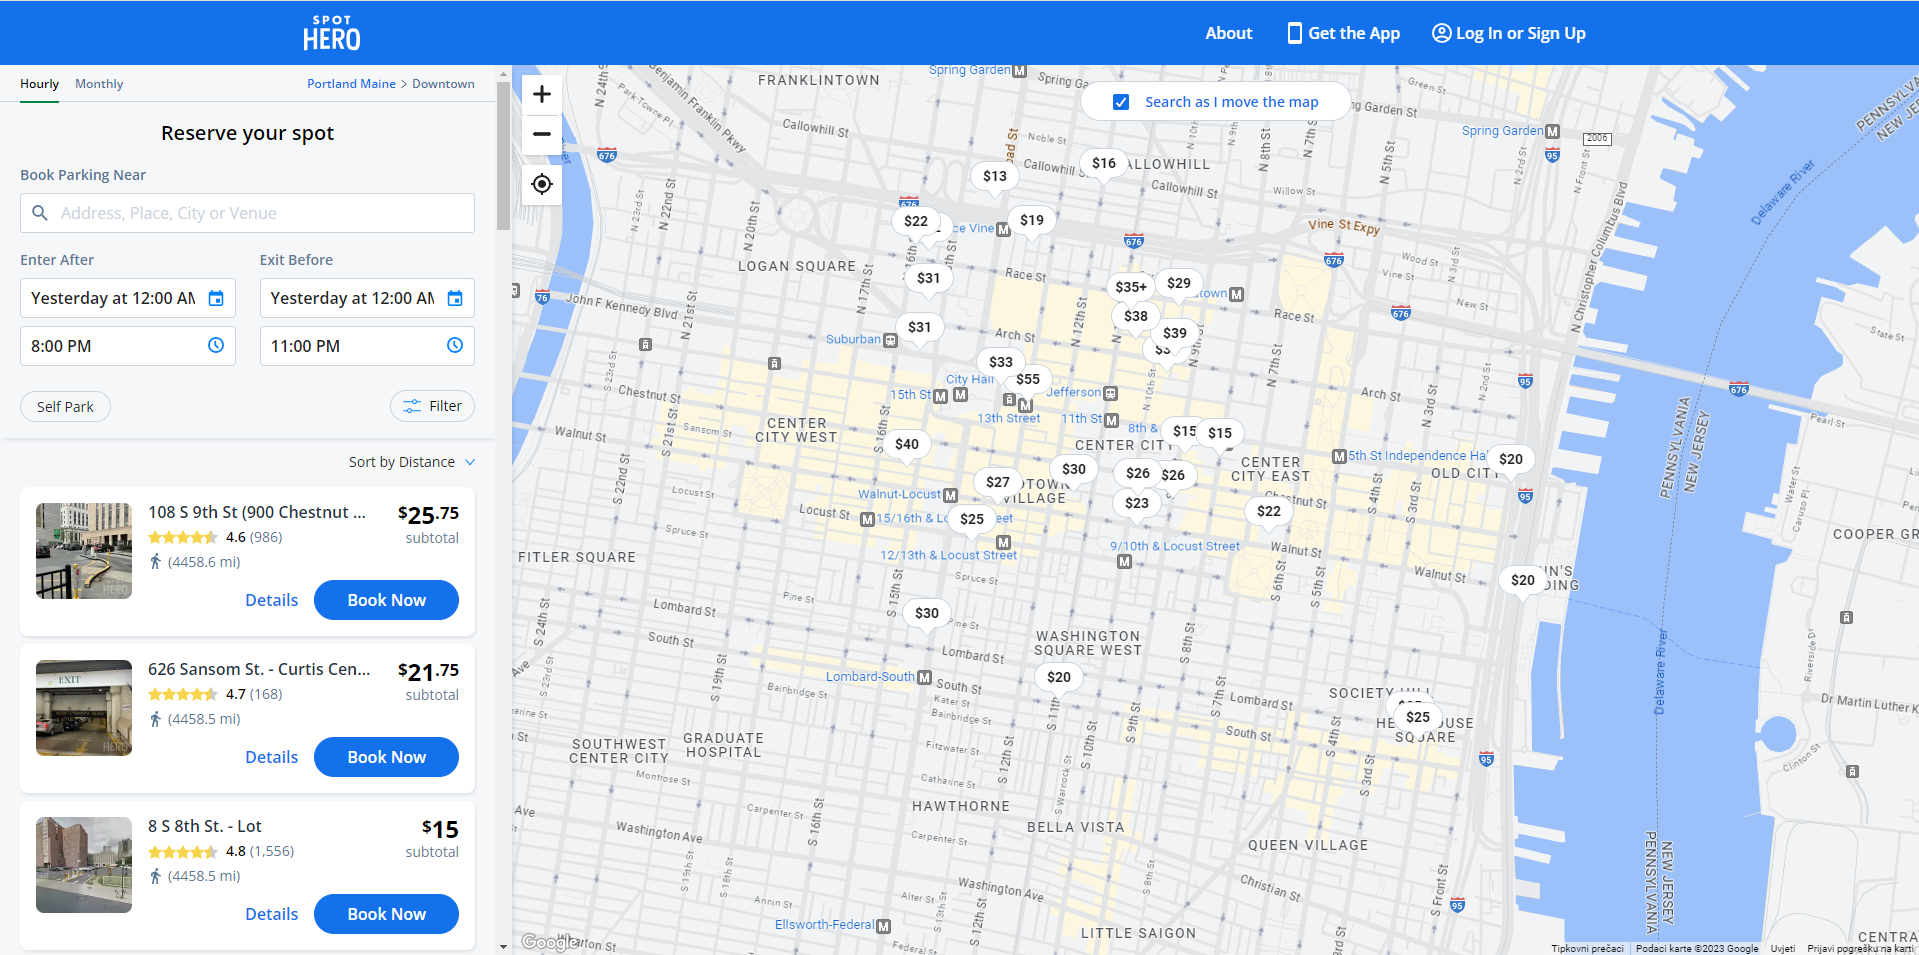
\includegraphics[width=\textwidth]{slike/spothero.PNG} 
			\caption{Prikaz aplikacije SpotHero}
			\label{fig:promjene3} 
		\end{figure}
		
		\begin{figure}[H]
			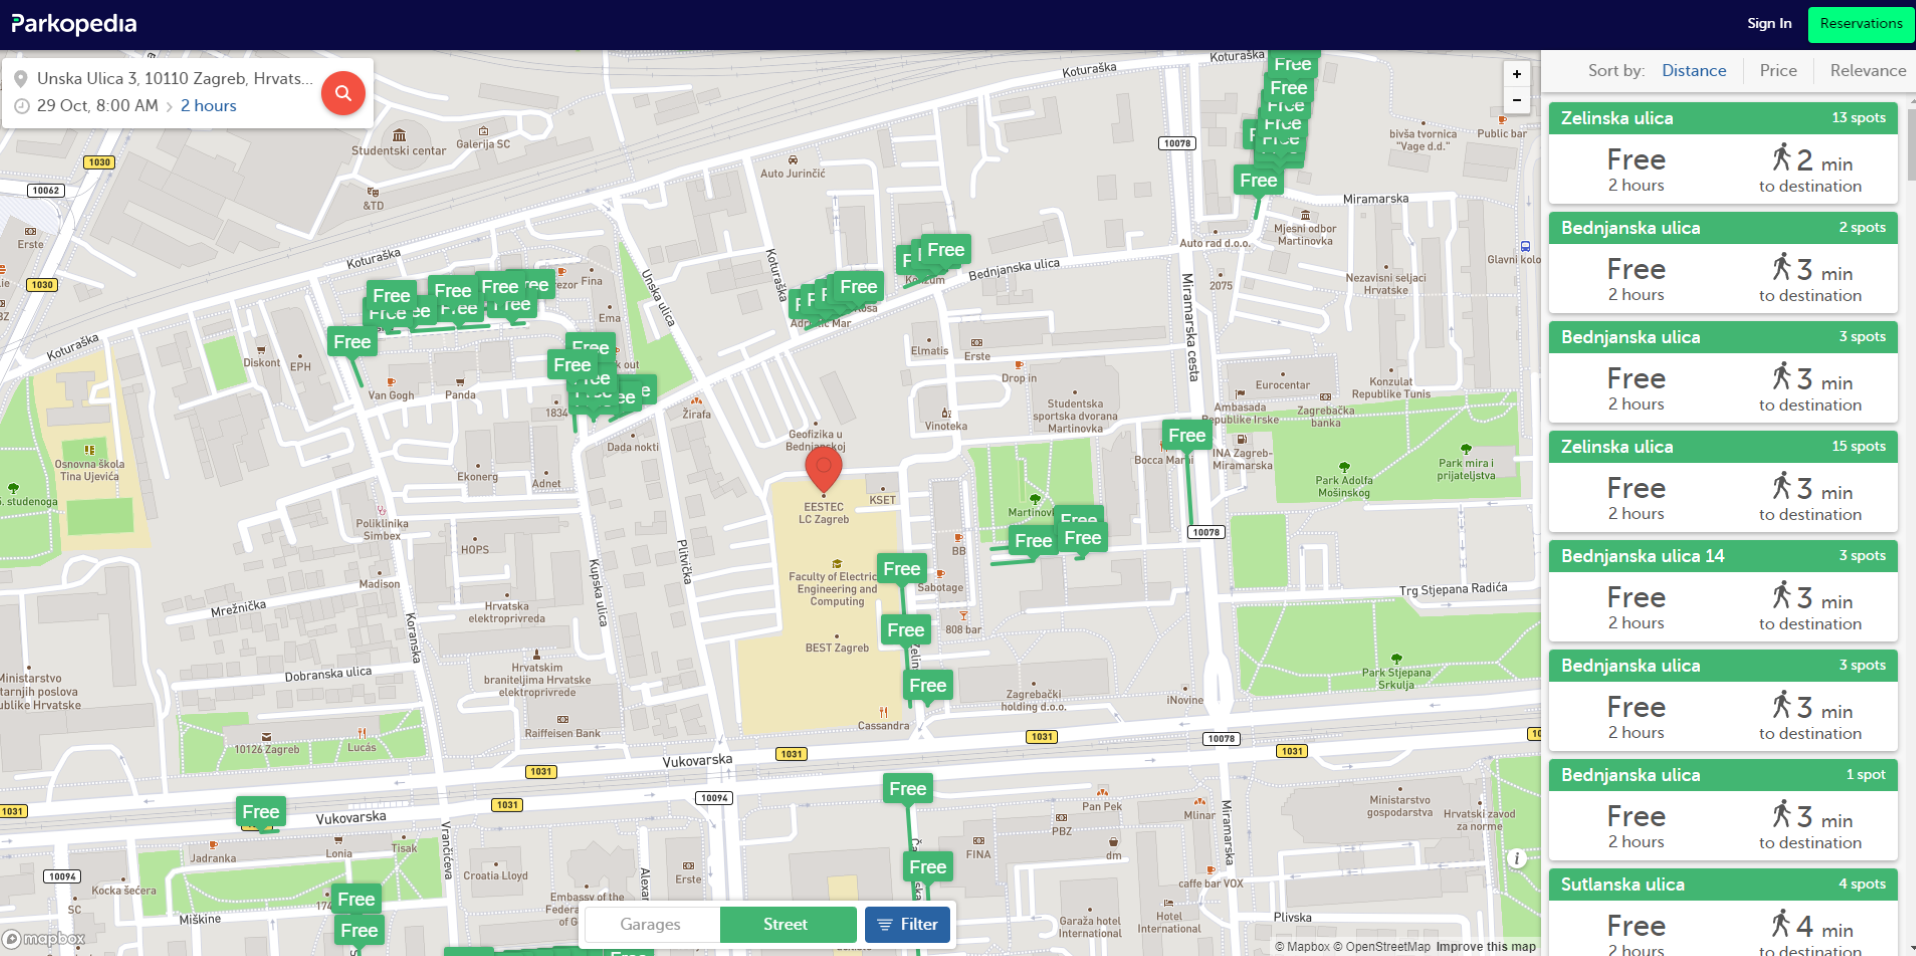
\includegraphics[width=\textwidth]{slike/parkopedia_street.PNG} 
			\caption{Prikaz aplikacije Parkopedia s označenim parkiralištima na ulici}
			\label{fig:promjene4} 
		\end{figure}
		
		\begin{figure}[H]
			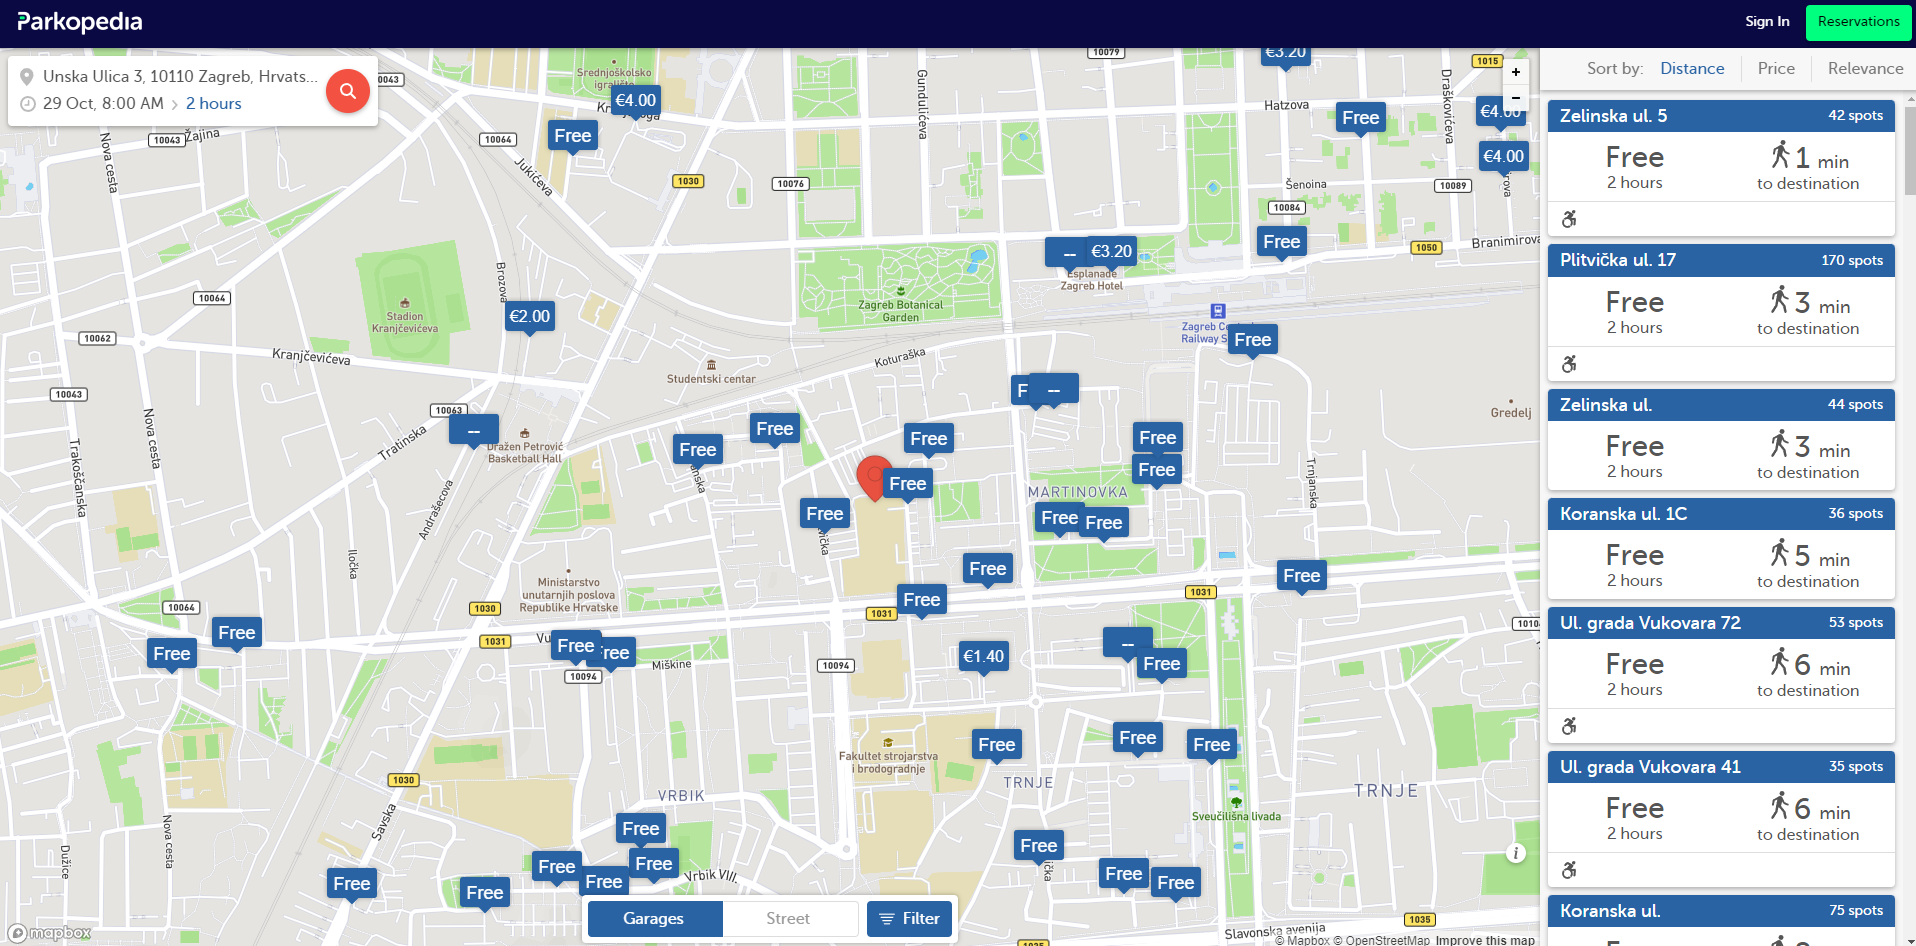
\includegraphics[width=\textwidth]{slike/parkopedia_garage.PNG}
			\caption{Prikaz aplikacije Parkopedia s označenim parkiralištima na garaži}
			\label{fig:promjene5} 
		\end{figure}
		
		Vjerujemo da našom aplikacijom možemo zainteresirati ljude koji su već upoznati s parking aplikacijama, ali smatraju da postoje područja u kojima trenutačno najpopularnije aplikacije nisu dovoljno prilagodljive korisničkim željama. Konačan plan i opseg ovog projekta je učiniti ovu aplikaciju dostupnu cijeloj Hrvatskoj. Ovisno o potrebi i potražnji korisnika, aplikaciju je moguće u budućnosti i nadograditi implementiranjem brojača slobodnih mjesta za bicikle.

		

		
	